\section{Agregar Medicamento}

Un medicamento es la parte medular de un tratamiento y no solo del tratamiento, si no de las notificaciones, es por eso que es tan importante el agregar un medicamento, para que se pueda trabajar con el tratamiento de forma activa y se puedan empezar a recibir las notificaciones que le recuerden al usuario cuando tomar sus medicinas.

\subsubsection{Procedimiento}
\begin{enumerate}
	
	\item Selecciona un tratamiento en estado activo de la pantalla \textbf{Tratamientos}.

	\begin{figure}[!htbp]			
		\hypertarget{fig:Tratamientos4}{\hspace{1pt}}
		\begin{center}
			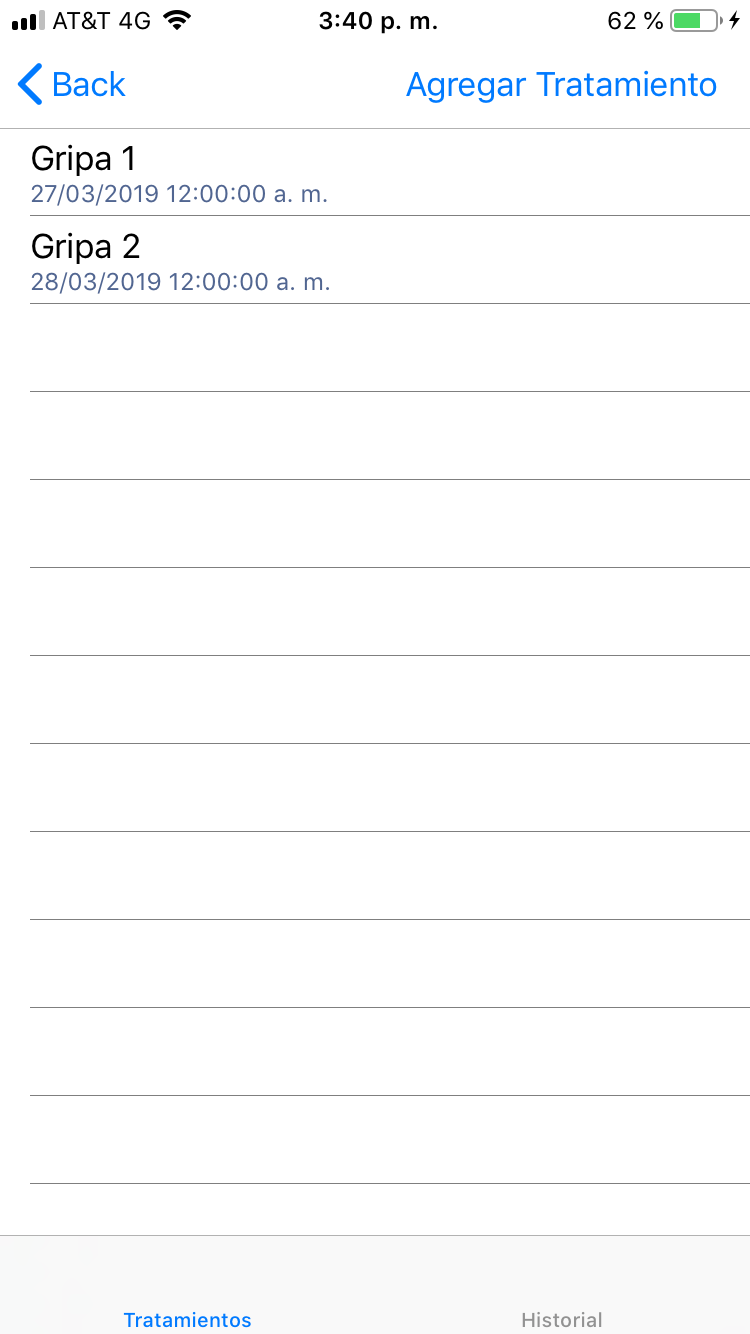
\includegraphics[height=0.4\textheight]{Paciente/AgregarMedicamento/images/Tratamientos}
			\caption{Tratamientos}
			\label{fig:Tratamientos4}
		\end{center}
	\end{figure}

	\item Se mostrará la pantalla \textbf{Información de Tratamiento}. 
	\newpage
	
	\begin{figure}[!htbp]			
		\hypertarget{fig:infoTratamiento2}{\hspace{1pt}}
		\begin{center}
			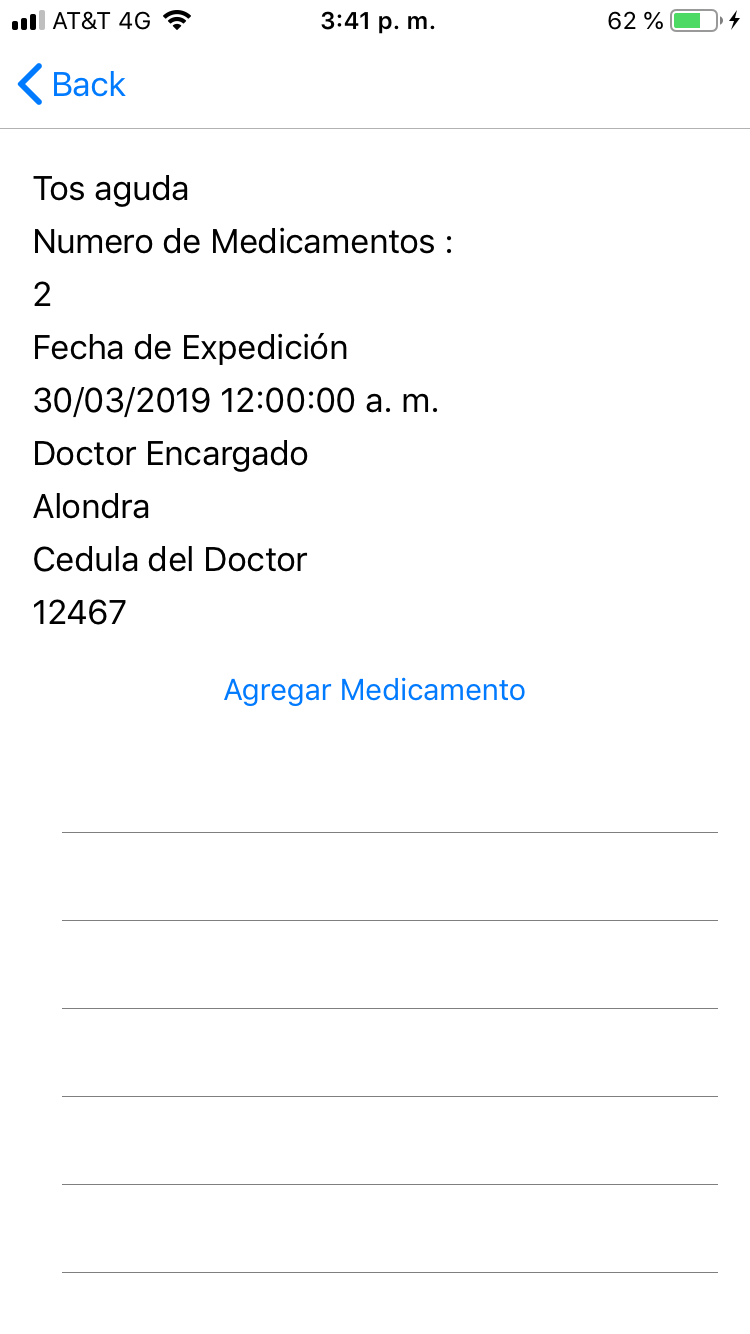
\includegraphics[height=0.4\textheight]{Paciente/AgregarMedicamento/images/infoTratamiento}
			\caption{Información de Tratamiento}
			\label{fig:infoTratamiento2}
		\end{center}
	\end{figure}

	\item Da clic en el botón \textbf{Agregar Medicamento} de la pantalla \textbf{Información de Tratamiento}.
	
	\item Se mostrará la pantalla \textbf{Agregar Medicina}
	\newpage
	\begin{figure}[!htbp]			
		\hypertarget{fig:AgregarMedicina}{\hspace{1pt}}
		\begin{center}
			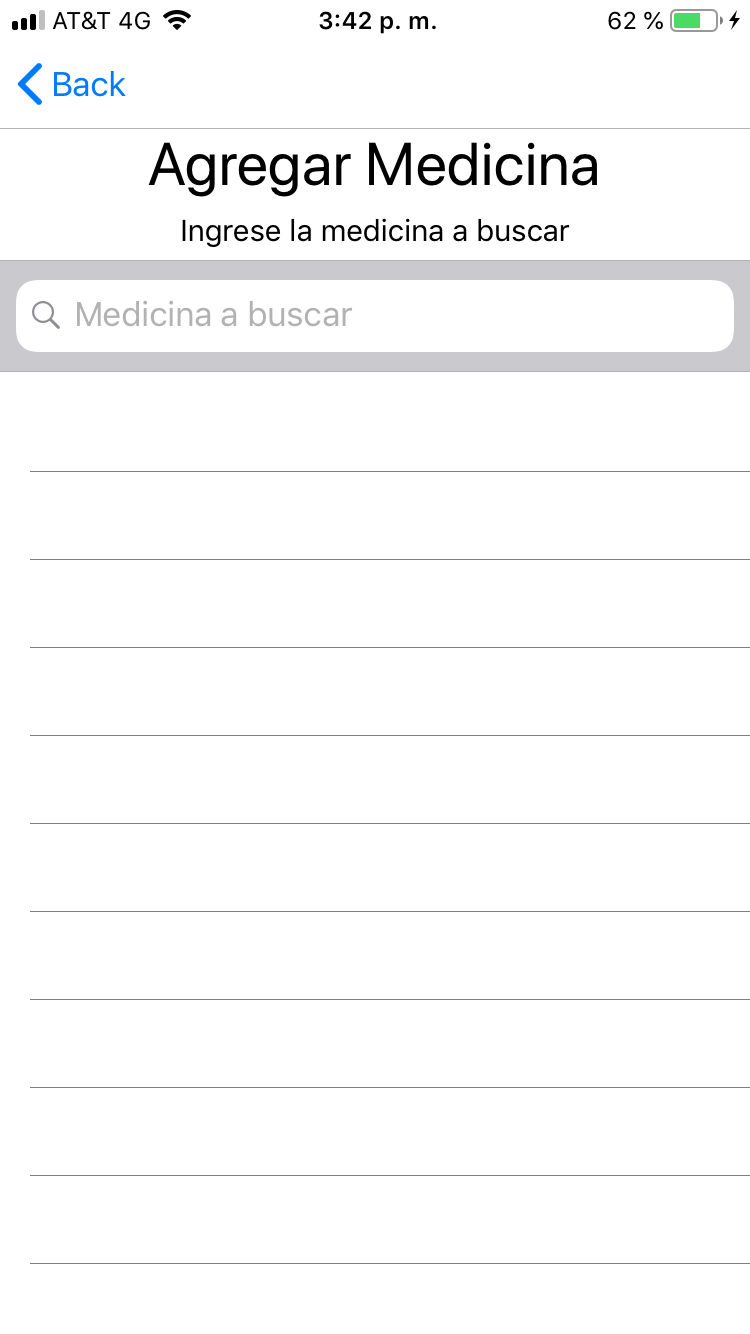
\includegraphics[height=0.4\textheight]{Paciente/AgregarMedicamento/images/AgregarMedicina}
			\caption{Agregar Medicina}
			\label{fig:AgregarMedicina}
		\end{center}
	\end{figure}

	\item Ingresa el nombre del medicamento.
	
	\item Selecciona el medicamento recetado por el Doctor.
	
	\item Ingresa el resto de los datos solicitados por la pantalla Agregar Medicina.
	\newpage
	\begin{figure}[!htbp]			
		\hypertarget{fig:AgregarMedicina2}{\hspace{1pt}}
		\begin{center}
			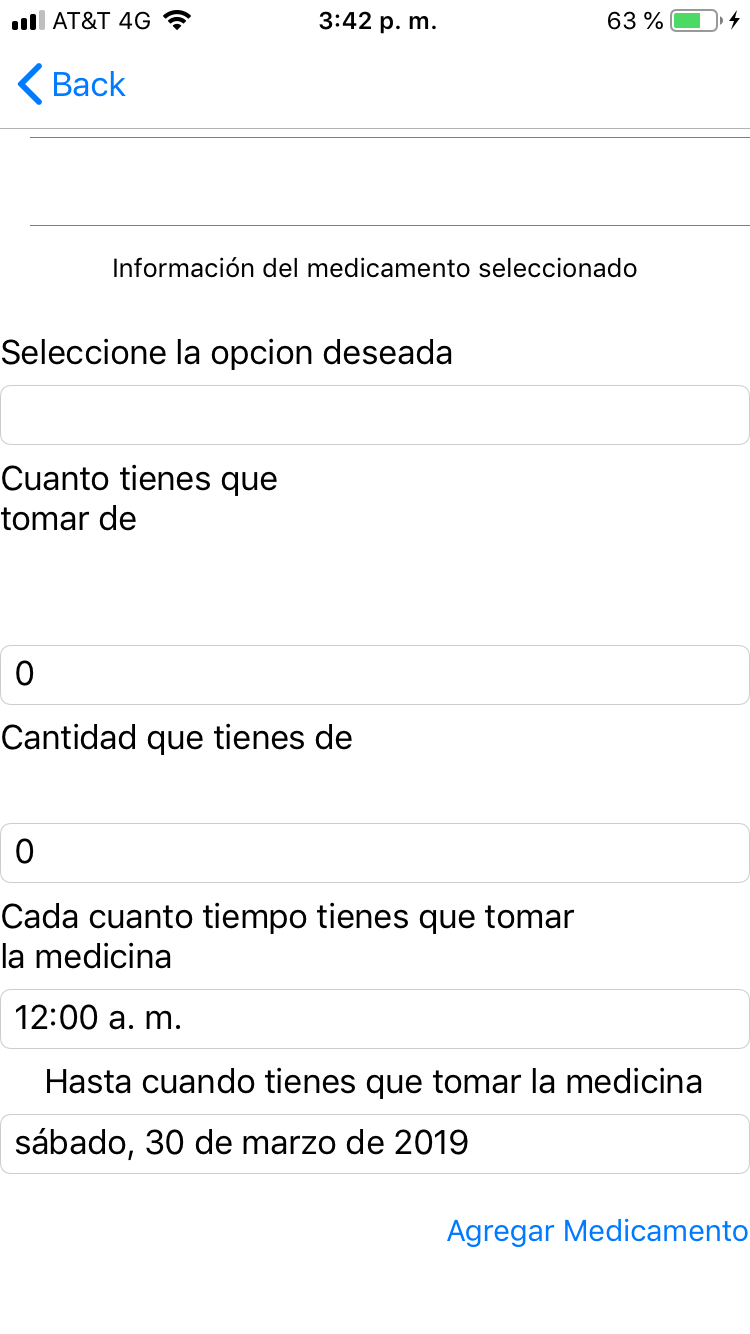
\includegraphics[height=0.4\textheight]{Paciente/AgregarMedicamento/images/AgregarMedicina2}
			\caption{Agregar Medicina}
			\label{fig:AgregarMedicina2}
		\end{center}
	\end{figure}
	
	\item Da clic en el botón \textbf{Agregar Medicamento}
	
	
\end{enumerate}

